\documentclass[watermark]{pbpreprint}
\usepackage{listings}
\usepackage[backend=biber,sorting=none]{biblatex}\addbibresource{bibliography.bib}
\usepackage{wasysym}

\newsubfloat{table}

\begin{document}
\title{The pharm\textcolor{uured}{b.io} preprint class}
\author{Jonathan Alvarsson}
\maketitle
\begin{KeepFromToc}
   \tableofcontents
\end{KeepFromToc}
\section{Regarding the use of the class}
\subsection{Required files}
The following files are needed in order to use the class:

\begin{table}[H]
    \centering
    \caption{The files needed to use the class}
    \begin{tabular}{ll}
    \toprule
    File name & Description \\
    \midrule
    \texttt{pbpreprint.cls} & The actual class file, always needed \\
    \texttt{figures/UU\_logo.pdf} & The Uppsala University logotype \\
    \texttt{figures/sigillnv.pdf} & The Uppsala University watermark \\
    \bottomrule
    \end{tabular}
\end{table}


\subsection{Class paramaters}
\begin{table}[H]
\caption{The class paramaters}
\centering
\begin{tabular}{lp{0.8\textwidth}}
    \toprule
    Paramater & Description \\
    \midrule
    \texttt{watermark} & Place the UU stamp in bottom right corner of the first
                         page and the UU logo above the title. \\ 
    \texttt{pad} & Adaptations for reading on digital device, changes page size and font to tgheros which is similar to helvetica \\
    \texttt{uu}        & Place the UU logo above the title \\
    \bottomrule
\end{tabular}
    \begin{flushleft}
        {\footnotesize \textsc{Note}: The UU watermark should only be used
                                      together with the normal UU logo.}
    \end{flushleft}
\end{table}

\subsection{About the class}
This is the pharm\textcolor{uured}{b.io} preprint class. It is meant to be used
for setting articles in a consistent way for preprint purposes but could also
be used for teaching materials an similar things. The class is based on the
\LaTeX\ Memoir class so everything that works with Memoir\footnote{Memoir
manual available from:
\url{http://texdoc.net/texmf-dist/doc/latex/memoir/memman.pdf}} shuld work
here. It uses the EB Garamond font\footnote{See:
\url{http://www.georgduffner.at/ebgaramond/}} which in the EB Garamond
project's own words: ``is an open source project to create a revival of Claude
Garamont’s famous humanist typeface from the mid-16th century.''

The class has a macro for making margin notes\note{This is a margin note //jonalv} and
another for making todos\todo{write what to do here}. This can be handy when
collaborating on a text or just for writing memos for one self.

It also uses EB Garamond for math type setting as can be seen here:
\begin{equation}
    \int_{a}^{b} x^2 dx + \frac{1}{2}
\end{equation}


\section{Some tips on the way}
The EBGaramond font contains both old style (\oldstylenums{0, 1, 2, 3, 4, 5, 6,
7, 8, 9}) numbers and lining numbers (\liningnums{0, 1, 2, 3, 4, 5, 6, 7, 8,
9}) default is old style. There is also tabular and propotional numbers where
tabular numbers are good for aligning numbers in tabels (see
Table~\ref{tabular}). Also remember to cite your
publications~\cite{spjuth2007bioclipse}.~\smiley{}


\begin{table}[h]
    \caption{Comparison of tabular nums and proportional numbers}
    \hfill
    \subtop[Tabular\label{tabular}]{\tabularnums{
        \begin{tabular}{lrr}
            \toprule
            Letter & Number & Number \\
            \midrule
            a &    123 &          45 \\
            b &     12 &           6 \\
            c & 1\,000 & 1\,100\,000 \\
            d & 5\,000 & 1\,123\,000 \\
            \bottomrule
        \end{tabular}
    }}
    \hfill
    \subtop[Proportional]{
        \begin{tabular}{lrr}
            \toprule
            Letter & Number & Number \\
            \midrule
            a &    123 &          45 \\
            b &     12 &           6 \\
            c & 1\,000 & 1\,100\,000 \\
            d & 5\,000 & 1\,123\,000 \\
            \bottomrule
        \end{tabular}
    }
    \hfill
\end{table}

\lstset{language=Tex, basicstyle=\ttfamily\scriptsize}
\begin{figure}
\begin{minipage}{0.49\textwidth}
\begin{lstlisting}
\begin{figure}
    \begin{center}
    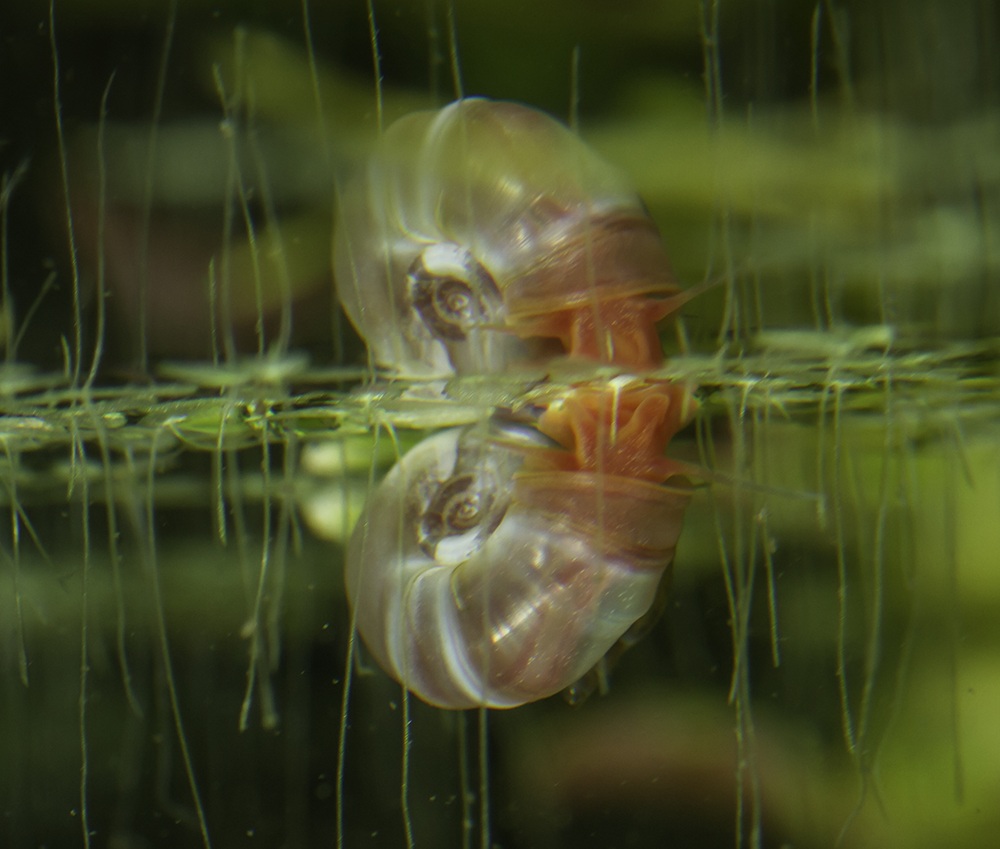
\includegraphics
      [width=0.7\textwidth]
      {figures/snail.png}
    \end{center}
    \caption{Snail on water surface}
\end{figure}
\end{lstlisting}
\end{minipage}
\hfill
\begin{minipage}{0.49\textwidth}
\begin{lstlisting}
    \begin{figure}
        \centering
        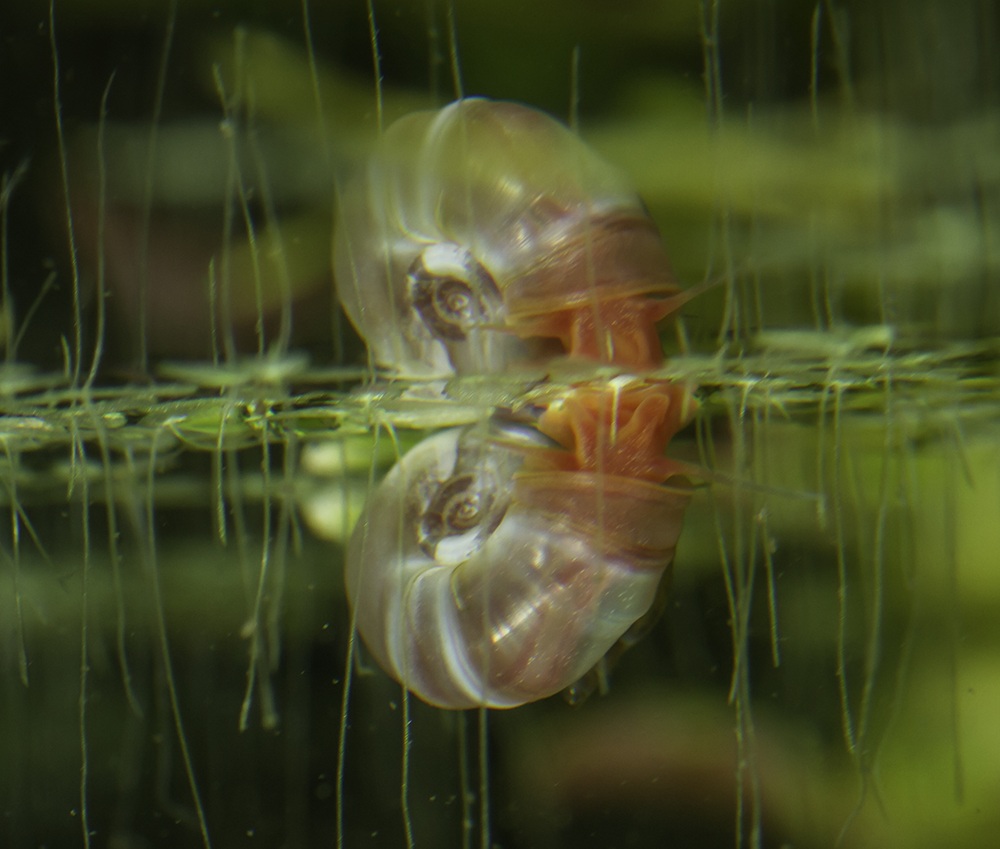
\includegraphics
          [width=0.7\textwidth]
          {figures/snail.png}
        \caption{Snail on water surface}
    \end{figure}
\end{lstlisting}
\end{minipage}

\fbox{\begin{minipage}[t]{0.44\textwidth}
    \begin{figure}[H]
        \begin{center}
        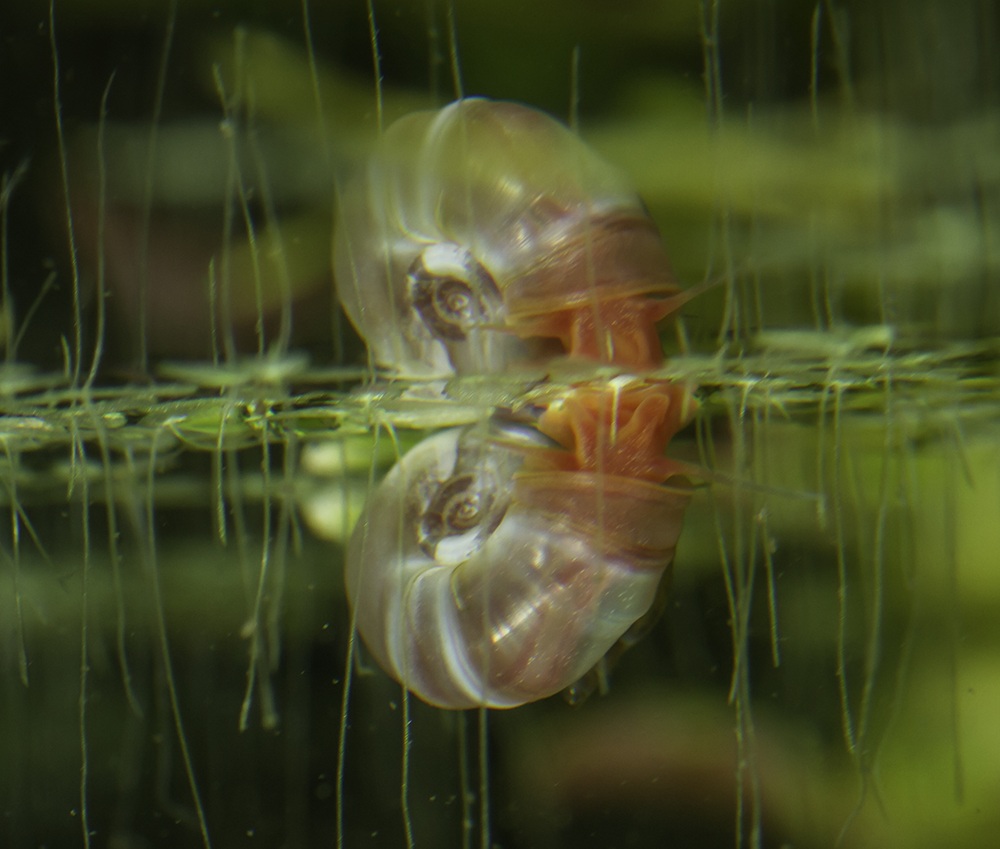
\includegraphics
          [width=0.7\textwidth]
          {figures/snail.png}
        \end{center}
        \caption{Snail on water surface}
    \end{figure}
\end{minipage}}
\hfill
\fbox{\begin{minipage}[t]{0.44\textwidth}
    \begin{figure}[H]
        \centering
        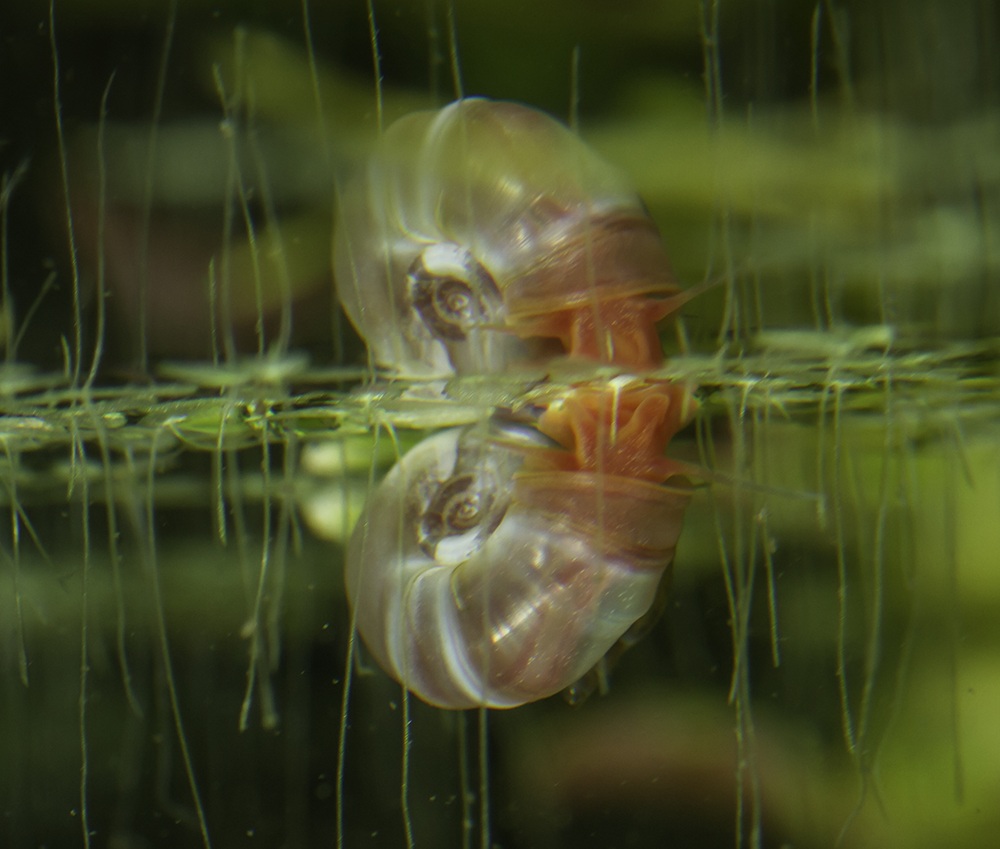
\includegraphics
          [width=0.7\textwidth]
          {figures/snail.png}
        \caption{Snail on water surface}
    \end{figure}
\end{minipage}}
\caption{In \texttt{\textbackslash figure} and \texttt{\textbackslash table} use \texttt{\textbackslash centering} instead of \texttt{\textbackslash begin\{center\}} because othewise you are adding extra space that shouldn't be there. Also, figure numbering is strange here because in order to show the extra space I wanted to use real figures which end up with their own numbers.}
\end{figure}

\printbibliography

\end{document}
